Completa la tabla \ref{tab:3.13}.

\begin{table}[H]
    \rowcolors{1}{}{lightgray!20}
    \centering
    \caption{Áreas}
    \label{tab:3.13}
    \begin{tabular}{|c|p{3cm}|c|p{3cm}|}
        \toprule
        \textbf{\color{white}Figura}                                     & \textbf{\color{white}Área} & \textbf{\color{white}Figura}                                     & \textbf{\color{white}Área} \\ \midrule
        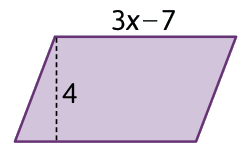
\includegraphics[width=0.1\linewidth]{../images/20230319042726}  & \ifprintanswers\fi         & 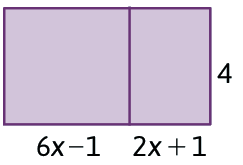
\includegraphics[width=0.13\linewidth]{../images/20230319042743} & \ifprintanswers\fi         \\ \hline
        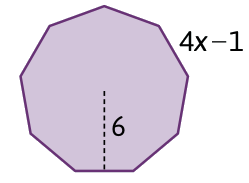
\includegraphics[width=0.14\linewidth]{../images/20230319042734} & \ifprintanswers\fi         & 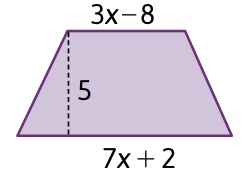
\includegraphics[width=0.18\linewidth]{../images/20230319042750} & \ifprintanswers\fi         \\ \hline
        \bottomrule
    \end{tabular}
\end{table}



